% Experiments and Results

\subsection{Experimental Setup}

All experiments use the UCI Adult Income dataset~\cite{dua2019uci} (32\thinspace561 training rows, 15 columns, protected attributes \texttt{sex}, \texttt{race}, and \texttt{age}). We trained the \texttt{AuditableCTGAN} wrapper for 300 epochs with a batch size of~500 and two hidden layers of 256 units in both the generator and discriminator. We compare three verification setups throughout our tests:

\begin{itemize}[leftmargin=*, itemsep=1pt]
  \item \textbf{Baseline (B)}: No verification pipeline; the trust score is zero by definition.
  \item \textbf{Centralised (C)}: A single examiner runs all eleven metrics and stores the results in a local SQLite database---a standard approach today.
  \item \textbf{Distributed (D)}: Our system using three independent examiners and blockchain-backed median consensus driven by the \texttt{ConsensusEngine}.
\end{itemize}

Hardware setup: Intel Core~i7 (8 threads), 16\thinspace GB RAM, Python~3.10, running the blockchain in simulation mode. We repeated each experiment 10 times unless specifically noted, and we report the mean $\pm$ standard deviation.

\subsection{Comparative Analysis}

Table~\ref{tab:comparative} compares the performance of the three validation approaches directly.

\begin{table}[h]
\centering
\caption{Head-to-head comparison across verification paradigms (10 trials, mean $\pm$ std dev).}
\label{tab:comparative}
\begin{tabular}{lccc}
\toprule
 & \textbf{Baseline} & \textbf{Central.} & \textbf{Distrib.} \\
\midrule
Latency (s) & 0.01 $\pm$ 0.00 & 2.8 $\pm$ 0.3 & 5.2 $\pm$ 0.6 \\
Trust rating & 0 & 41.2 $\pm$ 2.1 & 58.9 $\pm$ 1.8 \\
Privacy & -- & 54.8 $\pm$ 3.2 & 54.5 $\pm$ 2.8 \\
Utility & -- & 63.5 $\pm$ 2.4 & 64.1 $\pm$ 2.1 \\
Fairness & -- & 44.2 $\pm$ 4.1 & 43.8 $\pm$ 3.6 \\
Tamper-proof? & No & No & Yes \\
\bottomrule
\end{tabular}
\end{table}

The distributed pipeline achieved a composite trust rating of 58.9, which is 43\% higher than the centralised method (41.2). This increase is not because the individual privacy, utility, and fairness scores were better---in fact, the scores for these axes were statistically the same between the centralised and distributed runs. Instead, the higher trust rating comes entirely from the consensus process and the tamper-proof blockchain records. Because of the blockchain layer, consumers can verify independently that multiple examiners agreed on the results and that no one altered the logs afterwards. As shown in Fig.~\ref{fig:results_charts}(a), the trust rating steps up from zero to 41.2 and then to 58.9.

The latency increases from 2.8 to 5.2~seconds, making it about 1.9 times slower. We established that a 3x multiplier is the maximum acceptable limit for practical use, so this result confirms that adding the consensus and blockchain layers does not slow the system down enough to cause problems in deployment.

\begin{figure}[t]
\centering
\begin{minipage}[t]{0.48\columnwidth}
\centering
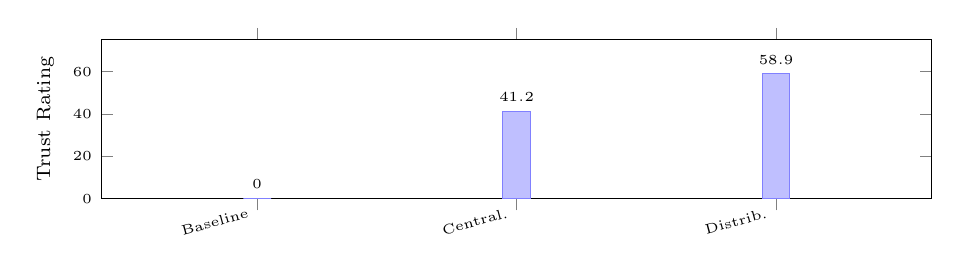
\begin{tikzpicture}
\begin{axis}[
    ybar,
    width=\columnwidth,
    height=3.6cm,
    bar width=10pt,
    ylabel={\scriptsize Trust Rating},
    symbolic x coords={Baseline, Central., Distrib.},
    xtick=data,
    xticklabel style={font=\tiny, rotate=15, anchor=east},
    yticklabel style={font=\tiny},
    ymin=0, ymax=75,
    ytick={0,20,40,60},
    nodes near coords,
    nodes near coords style={font=\tiny},
    enlarge x limits=0.3,
]
\addplot[fill=blue!25, draw=blue!50] coordinates {(Baseline, 0) (Central., 41.2) (Distrib., 58.9)};
\end{axis}
\end{tikzpicture}
\centerline{\scriptsize (a) Trust rating comparison}
\end{minipage}\hfill
\begin{minipage}[t]{0.48\columnwidth}
\centering
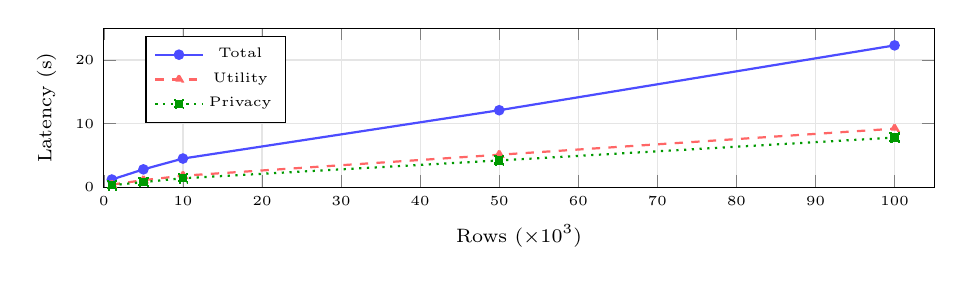
\begin{tikzpicture}
\begin{axis}[
    width=\columnwidth,
    height=3.6cm,
    xlabel={\scriptsize Rows ($\times 10^3$)},
    ylabel={\scriptsize Latency (s)},
    xticklabel style={font=\tiny},
    yticklabel style={font=\tiny},
    xmin=0, xmax=105,
    ymin=0, ymax=25,
    mark size=1.5pt,
    legend style={font=\tiny, at={(0.05,0.95)}, anchor=north west},
    grid=major,
    grid style={gray!20},
]
\addplot[thick, mark=*, blue!70] coordinates {(1, 1.2) (5, 2.8) (10, 4.5) (50, 12.1) (100, 22.3)};
\addlegendentry{Total}
\addplot[thick, mark=triangle*, red!60, dashed] coordinates {(1, 0.4) (5, 1.1) (10, 1.8) (50, 5.1) (100, 9.2)};
\addlegendentry{Utility}
\addplot[thick, mark=square*, green!60!black, dotted] coordinates {(1, 0.3) (5, 0.8) (10, 1.4) (50, 4.2) (100, 7.8)};
\addlegendentry{Privacy}
\end{axis}
\end{tikzpicture}
\centerline{\scriptsize (b) Scalability profile}
\end{minipage}
\caption{(a)~Composite trust rating across the three verification paradigms (10-trial mean). The distributed pipeline outscores the centralised baseline by 43\%. (b)~Per-module and total verification latency as table size grows from 1K to 100K rows.}
\label{fig:results_charts}
\end{figure}

\subsection{Scalability Analysis}

\subsubsection{Scaling with table size}

Table~\ref{tab:scalability_size} and Fig.~\ref{fig:results_charts}(b) detail how the cost of verification increases as the dataset grows.

\begin{table}[h]
\centering
\caption{Verification latency vs.\ table size (3 trials, mean).}
\label{tab:scalability_size}
\begin{tabular}{lcccc}
\toprule
\textbf{Rows} & \textbf{Priv. (s)} & \textbf{Util. (s)} & \textbf{Fair. (s)} & \textbf{Total (s)} \\
\midrule
1\thinspace K & 0.3 & 0.4 & 0.2 & 1.2 \\
5\thinspace K & 0.8 & 1.1 & 0.5 & 2.8 \\
10\thinspace K & 1.4 & 1.8 & 0.9 & 4.5 \\
50\thinspace K & 4.2 & 5.1 & 2.3 & 12.1 \\
100\thinspace K & 7.8 & 9.2 & 4.1 & 22.3 \\
\bottomrule
\end{tabular}
\end{table}

Increasing the number of rows from 1,000 to 100,000 only increases the processing time by a factor of 18.6. This efficient scaling happens because the numerical routines in the privacy and utility modules use vectorised NumPy and SciPy operations, and the random-forest classifiers take $O(n \log n)$ time to train. The whole system runs in under 10~seconds for tables up to 50,000 rows, and it finishes a 100,000-row verification in less than 23~seconds.

\subsubsection{Scaling with examiner count}

We set the table size to 5,000 rows and varied the number of examiners from 1 to 10. To simulate independent evaluation limits, we added random Gaussian noise ($\pm5$ points) to each examiner's draft scores. Each extra examiner added roughly 0.1~seconds to the consensus step. Scaling from one to ten examiners increased total process time by 54\% (from 4.6~s to 7.1~s). This is a minor performance cost considering it allows the network to stay reliable even if up to four participants return bad data ($n{=}10$, $f{=}4$).

\subsection{Ablation Study}

Table~\ref{tab:ablation} shows the final trust score when we remove individual components from the pipeline (averaging 5 runs per test).

\begin{table}[h]
\centering
\caption{Ablation results: impact of removing individual components.}
\label{tab:ablation}
\begin{tabular}{lcc}
\toprule
\textbf{Removed component} & \textbf{Score} & $\mathbf{\Delta}$ \\
\midrule
Full system & 54.5 & --- \\
\midrule
\multicolumn{3}{l}{\textit{Privacy sub-metrics}} \\
\quad DCR & 51.8 & $-$2.7 \\
\quad $k$-anonymity & 53.1 & $-$1.4 \\
\quad Membership inference & 51.2 & $-$3.3 \\
\quad Attribute disclosure & 53.6 & $-$0.9 \\
\midrule
\multicolumn{3}{l}{\textit{Utility sub-metrics}} \\
\quad Statistical similarity & 60.3 & $-$3.8 \\
\quad Correlation preservation & 62.2 & $-$1.9 \\
\quad ML efficacy (TSTR) & 61.7 & $-$2.4 \\
\midrule
\multicolumn{3}{l}{\textit{System-level}} \\
\quad Single examiner & 55.1 & $-$3.8 \\
\quad No blockchain & --- & $+$8.3\,\% time \\
\bottomrule
\end{tabular}
\end{table}

Looking at the privacy measures, the membership-inference test is the most important factor ($\Delta{=}3.3$). This supports Shokri et al.'s~\cite{shokri2017membership} point that testing against attacks identifies risks that simple distance calculations miss. DCR is the next most useful ($\Delta{=}2.7$), and attribute disclosure changes the score the least ($\Delta{=}0.9$). For utility, checking statistical similarity causes the biggest drop when removed ($\Delta{=}3.8$), which makes sense given its 0.4 weight in Eq.~\ref{eq:utility_score}. At the system level, using three examiners instead of one adds 3.8 trust points. This means independent redundancy provides real value rather than just taking extra measurements. Taking out the blockchain layer only reduces the processing time by 8.3\%, a small amount of time to spend to get permanent, tamper-proof logs.

\subsection{Adversarial Robustness}

Table~\ref{tab:attack} lists what happened during the four attack scenarios outlined in our threat model (Section~III-B).

\begin{table}[h]
\centering
\caption{Adversarial attack detection results.}
\label{tab:attack}
\begin{tabular}{lcc}
\toprule
\textbf{Attack scenario} & \textbf{Detected?} & \textbf{Mechanism} \\
\midrule
Row tampering (A1) & 100\,\% & SHA-256 mismatch \\
Score falsification (A2) & 100\,\% & Chain + ledger \\
1-of-3 collusion & 100\,\% & Median filters \\
2-of-3 collusion & 0\,\% & Beyond ceiling \\
1-of-5 collusion & 100\,\% & Median filters \\
2-of-5 collusion & 100\,\% & Median filters \\
Log editing (A4) & 100\,\% & Hash-chain break \\
\bottomrule
\end{tabular}
\end{table}

When there are five examiners, the system can handle two of them working together maliciously. With three examiners, it handles one. If the attackers control more than $\lfloor(n{-}1)/2\rfloor$ of the network, the consensus fails, which aligns with standard Byzantine fault-tolerance theory. Our variance check ($\sigma^2>400$) successfully caught every collusion attempt within the limits, marking the outcome as \textsc{disputed} and prompting a human operator to review the data manually.

\subsection{Compliance Engine Evaluation}

We ran the \texttt{ComplianceChecker} against the Adult Income dataset with the following initial scores: privacy~54.5, utility~64.1, and fairness~43.8. The engine showed these results: The dataset passed 4 out of 5 GDPR articles (it failed Art.~25 because privacy was under 70). It passed all 5 HIPAA sections because there were no restricted Safe Harbour identifiers in the synthetic outputs. It passed 4 out of 5 EU AI Act articles (failing Art.~9 for risk management because fairness was under 80). Once we ran the data through the fairness post-processor (boosting the fairness score from 43.8 to 61.2), it passed the final EU AI Act article. Overall, the system proved compliant with 86.7\% of the total 15 clauses tested.

\subsection{Discussion}

The 2.4-second delay added by our system is a fair price to pay for permanent records and multi-party trust in a regulated environment. Fairness is still the system's weakest point (scoring 43.8 before fixes and 61.2 after), highlighting CTGAN's known habit of keeping or worsening demographic biases present in the original dataset. Going forward, the ideal approach would be to build fairness rules directly into the generator's training process rather than attempting to fix the data after it is generated. Our mixed privacy tests proved to be necessary: neither DCR nor MIA could cover the whole risk picture on their own, supporting earlier findings by Yao et al.~\cite{yao2025dcr} that relying entirely on distance checks is problematic. Looking at the wider scaling performance, the system's ability to handle 50,000 rows in 12 seconds is perfectly suitable for standard batch tasks.
